\section{Vorbereitende Arbeiten}
\subsection{Analytische Modellierung eines DC-Motors}
\subsubsection{Bestimmung der Übertragungsfunktionen}
Die erste Aufgabe besteht darin, zwei Übertragungsfunktionen eines typischen DC-Motors an Hand eines White Box Modellings zu bestimmen.
Abbildung \ref{fig:SchemaDCSystem} zeigt schematisch das DC-System, wobei sowohl das Massenträgheitsmoment $J_{\text{load}}$ als auch die viskose Reibung $b_{\text{load}}$ der Last mit null angenommen werden können.
\begin{figure}[H]
    \centering
    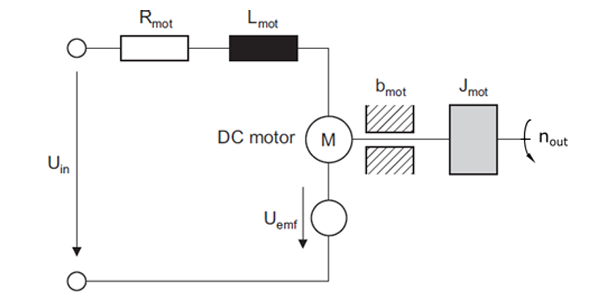
\includegraphics[width=0.6\textwidth]{images/LabDC_SchemaDCSystem.png}
    \caption[Schema des DC-Systems]{Schematische Repräsentation des elektro-mechanischen Systems.}
    \label{fig:SchemaDCSystem}
\end{figure}

Dabei sollen folgende Übertragungsfunktionen bestimmt werden:
\begin{equation}
    \label{eq:DC_TransferFunctions}
    G_{\text{p1}}(s) = \frac{Angular Displacement(s)}{Voltage(s)} = \frac{\Theta(s)}{U_{in}(s)}
\end{equation}
\begin{equation}
    \label{eq:DC_TransferFunctions2}
    G_{\text{p2}}(s) = \frac{Angular Velocity(s)}{Voltage(s)} = \frac{\Omega(s)}{U_{in}(s)}
\end{equation}
Die Gleichungen des Systems können durch die Anwendung der Kirchhoff'schen Gesetze und der mechanischen Gleichungen abgeleitet werden.
Die elektrische Gleichung des Systems lautet:
\begin{equation}
    \label{eq:DC_ElectricalEquation}
    U_{in} = R_{mot} \cdot i + L_{mot} \cdot \frac{di}{dt} + U_{emf}
\end{equation}
Wobei die Spannung $U_{emf}$ durch die Gleichung
\begin{equation}
    \label{eq:DC_EMF}
    U_{emf} = k_e \cdot \dot{\theta}
\end{equation}
beschrieben wird. Die mechanische Gleichung des Systems lautet, wenn $J_{load}=0,\ b_{load}=0$ angenommen werden:
\begin{equation}
    \label{eq:DC_MechanicalEquation}
    J_{mot} \cdot \ddot{\theta} = k_t \cdot i - b_{mot} \cdot \dot{\theta}
\end{equation}

Um aus den Grundgleichungen \ref{eq:DC_ElectricalEquation} und \ref{eq:DC_MechanicalEquation} die Transferfunktionen zu erhalten, werden die Gleichungen in den Laplace-Raum transformiert:
\newline
Elektrisch: 
\begin{equation}
    \label{eq:DC_ElectricalEquationLaplace}
    \quad U_{in}(s) = (R_{mot} + L_{mot} s) \cdot I(s) + k_e s \cdot \Theta(s)
\end{equation}
Mechanisch: 
\begin{equation}
    \label{eq:DC_MechanicalEquationLaplace}
    \quad I(s) = \frac{J_{mot} s^2 + b_{mot} s}{k_t} \cdot \Theta(s)
\end{equation}

Danach wird die  Gleichung \ref{eq:DC_ElectricalEquationLaplace} nach $I(s)$ und die zweite Gleichung \ref{eq:DC_MechanicalEquationLaplace} nach $\Theta(s)$ aufgelöst, um die Transferfunktion \ref{eq:DC_TransferFunctions} zu erhalten:
\begin{equation}
    \label{eq:DC_TransferFunction1_final}
    G_{p1}(s) = \frac{k_t}{s \cdot (L_{mot} \cdot J_{mot} \cdot s^2 + (R_{mot} \cdot J_{mot} + L_{mot} \cdot b_{mot}) \cdot s + (R_{mot} \cdot b_{mot} + k_e \cdot k_t))}
\end{equation}

Der Faktor $s$ im Nenner entspricht dem Integrierer, da die reine Rotation ohne Rückstellkraft betrachtet wird.
Daraus folgt:
\begin{equation}
    \label{eq:DC_TransferFunction_step}
    \Omega(s) = s\cdot\Theta(s)
\end{equation}
Somit kann die zweite Übertragungsfunktion \ref{eq:DC_TransferFunctions2} aus der ersten finalen Transferfunktion, die in Gleichung \ref{eq:DC_TransferFunction1_final} beschrieben ist, bestimmt werden:
\begin{equation}
    \label{eq:DC_TransferFunction2_final}
    G_{p2}(s) = \frac{k_t}{L_{mot} \cdot J_{mot} \cdot s^2 + (R_{mot} \cdot J_{mot} + L_{mot} \cdot b_{mot}) \cdot s + (R_{mot} \cdot b_{mot} + k_e \cdot k_t)}
\end{equation}

\subsubsection{Aufstellen des State-Space Modells}
Ausgehend von $G_{p1}$, Gleichung \ref{eq:DC_TransferFunction1_final}, kann das State-Space Modell des Systems aufgestellt werden. Dazu werden die Zustandsvariablen definiert als:
\begin{equation}
    \label{eq:DC_StateVariables}
    x_1 = \theta, \quad x_2 = \dot{\theta}, \quad x_3 = i
\end{equation}

Die Zustandsraumdarstellung des Systems kann dann in der Form
\begin{align}
    \dot{\mathbf{x}}(t) &= \mathbf{A} \mathbf{x}(t) + \mathbf{B} u(t) \\
    y(t) &= \mathbf{C} \mathbf{x}(t) + \mathbf{D} u(t)
\end{align}
aufgestellt werden, wobei $\mathbf{x}(t) = [x_1(t), x_2(t), x_3(t)]^T$ der Zustandsvektor, $u(t)$ die Eingangsgröße und $y(t)$ die Ausgangsgröße ist.
Die Matrizen $\mathbf{A}$, $\mathbf{B}$, $\mathbf{C}$ und $\mathbf{D}$ können durch die Umformung der Gleichungen \ref{eq:DC_ElectricalEquation} und \ref{eq:DC_MechanicalEquation} in die Zustandsraumdarstellung bestimmt werden. 
Die aus den physikalischen Gleichungen resultierenden Zustandsgleichungen lauten:
\begin{equation}
    \label{eq:DC_StateSpaceEquations}
    \dot{x}_1 = x_2 , \quad \dot{x}_2 = -\frac{b_{mot}}{J_{mot}}x_2 + \frac{k_t}{J_{mot}}x_3, \quad \dot{x}_3 = -\frac{k_e}{L_{mot}}x_2 - \frac{R_{mot}}{L_{mot}}x_3 + \frac{1}{L_{mot}}U_{in}
\end{equation}

In der Matrixdarstellung ergibt sich somit die folgende Form für die Matrizen $\mathbf{A}$, $\mathbf{B}$, $\mathbf{C}$ und $\mathbf{D}$:
\begin{equation}
    \label{eq:DC_StateSpaceMatrices}
    \mathbf{A} = \begin{pmatrix} 0 & 1 & 0 \\ 0 & -\dfrac{b_{mot}}{J_{mot}} & \dfrac{k_t}{J_{mot}} \\ 0 & -\dfrac{k_e}{L_{mot}} & -\dfrac{R_{mot}}{L_{mot}} \end{pmatrix}, \quad \mathbf{B} = \begin{pmatrix} 0 \\ 0 \\ \dfrac{1}{L_{mot}} \end{pmatrix}, \quad \mathbf{C} = \begin{pmatrix} 1 & 0 & 0 \end{pmatrix}, \quad \mathbf{D} = 0
\end{equation}
Das resultierende State-Space Modell ermöglicht nun die Analyse und das Design von Regelungsstrategien für das DC-System.


\subsection{Identifikation der Systemparameter}
WIE REFERENZIEREN WIR HIER DIE DATEN UND DAS MATLAB-SKRIPT
\newline
Aus der von der LV-Leiterung bereitgestellten Datei measurement\_data und dem Matlab Skript prepWork32 konnte folgende Abbildung erstellt werden.
\begin{figure}[H]
    \centering
    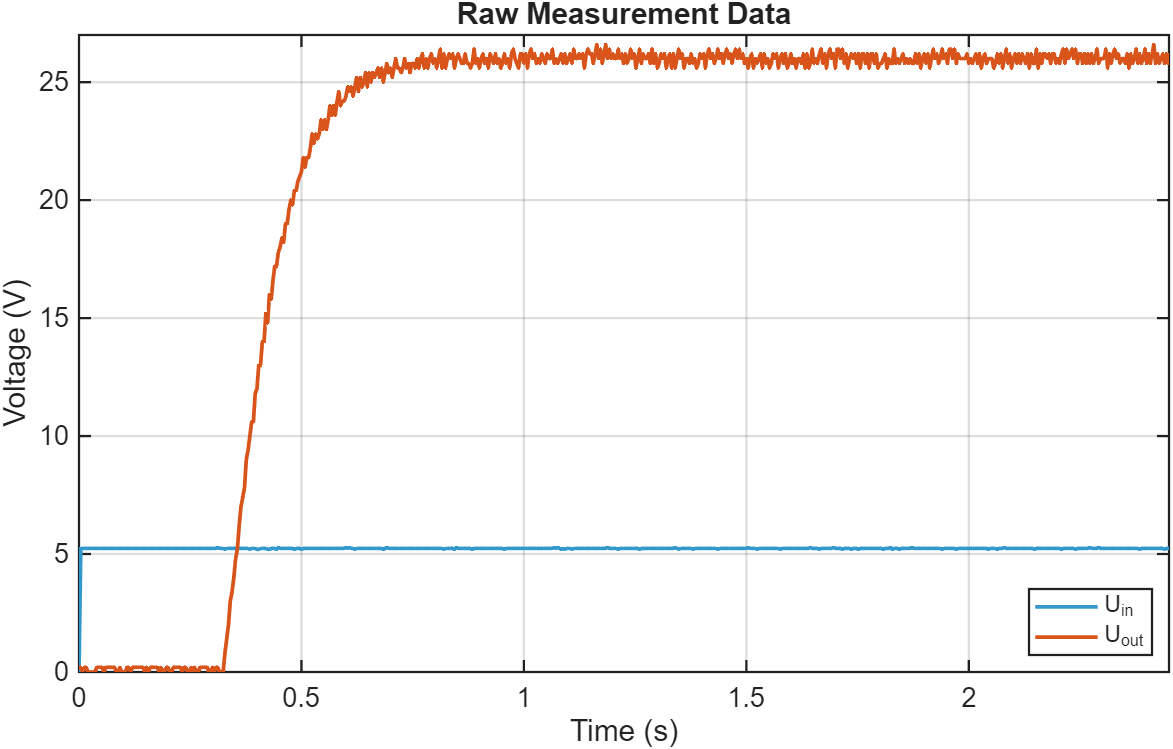
\includegraphics[width=0.6\textwidth]{images/Plot_rawData.png}
    \caption[PlotRawData]{Rohdaten der Step Response.}
    \label{fig:PlotRawData}
\end{figure}
Abbildung \ref{fig:PlotRawData} zeigt die Rohdaten der Step Response des Systems, welche durch die Anwendung einer Spannung von fünf Volt aufgenommen wurden. 
Die Rohdaten zeigen eine typische S-Kurve, welche auf ein PT2-System hindeutet. Dabei spiegelt der Plot nicht hundertprozentig die in den Laborinstructions \cite{labinstruction2026} vorgegebene Kurve, da in den Rohdaten bereits der Delay von 0,8 Sekunden entfernt wurde.

\begin{figure}[H]
    \centering
    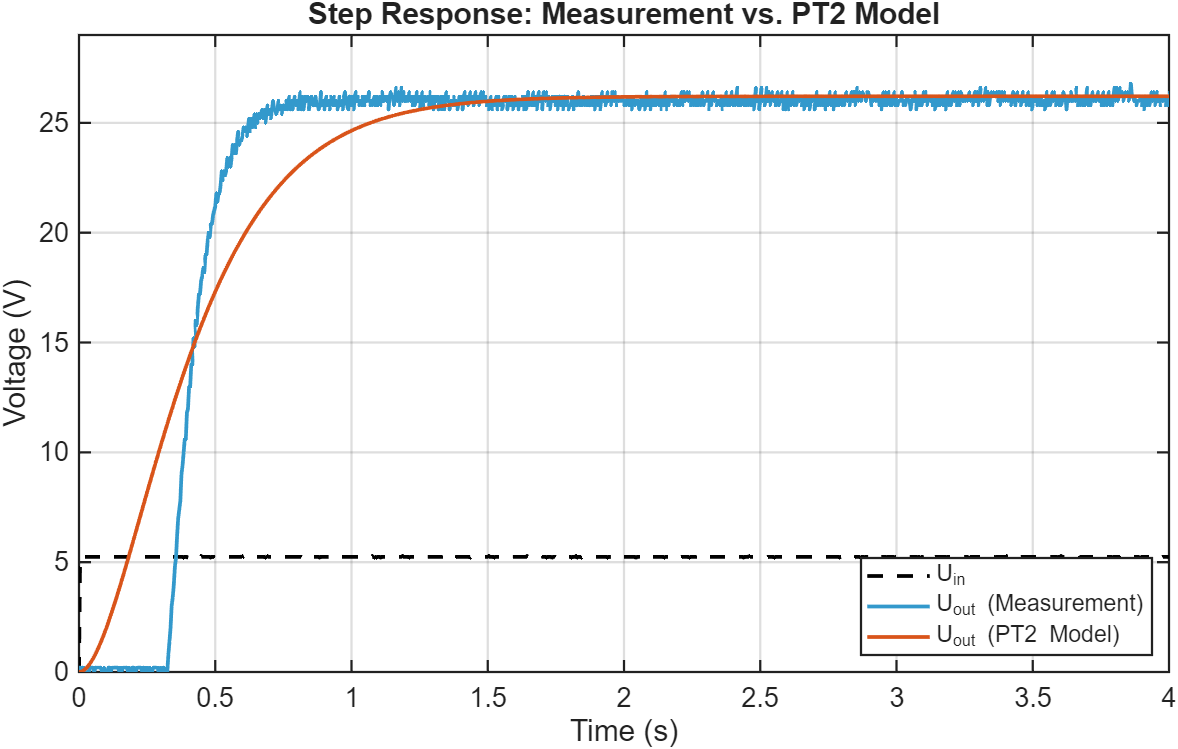
\includegraphics[width=0.6\textwidth]{images/Vergleich_rawDataPT2.png}
    \caption[rawDataPT2]{Vergleich der Rohdaten mit gefitteten PT2-Modell.}
    \label{fig:rawDataPT2}
\end{figure}
In Abbildung \ref{fig:rawDataPT2} ist ein Vergleich der Rohdaten mit dem gefitteten PT2-Modell zu sehen. Die Übertragungsfunktion wurde anhand von lsqcurvfit bestimmt, sodass die folgende Transferfunktion des PT2-Systems erhalten wurde:
\begin{equation}
    \label{eq:PT2_TransferFunction}
    G_\text{PT2}(s) = \frac{5.002}{0.04883s^2 + 0.442s + 1}
\end{equation}